\chapter{Referencial Tecnológico} 
    \label{chap:ReferencialTecnologico}

Nesse capítulo, serão acordados as principais tecnologias e suportes, no intuito de realizar o trabalho em termos de \nameref{pesquisa}, \nameref{desenvolvimento} e \nameref{complementar}. Por fim, tem-se o \nameref{resumo}.

%%%%%%%%%%%%%%%%%%%%%%%%%%%%%%%%%%%%%%%%%%%%%%%%%%%%

\section{Apoio à Pesquisa} 
    \label{pesquisa}

Visando realizar a pesquisa, são necessárias ferramentas que viabilizem buscas por artigos e materiais de interesse, bem como a elaboração e hospedagem de questionários. 

Para o caso das buscas por artigos e demais materiais de cunho investigativo, foram utilizadas as bases científicas ScienceDirect (Elsevier), IEEE, bem como o Google Acadêmico disponíveis através do Periódicos Capes. Detalhes complementares sobre essas buscas constam no Método de Pesquisa, disponível no \hyperref[chap:Metodologia]{Capítulo 4 - Metodologia}.

Para o caso da elaboração e hospedagem de questionários, estão sendo utilizados \nameref{GoogleForms} e \nameref{GoogleSheets}. Tais suportes estão auxiliando nos levantamentos realizados ao longo da pesquisa, seja para identificação plataformas comumente utilizadas em comércio eletrônico móvel, seja para fins de avaliação junto aos usuários.

%%%%%%%%%%%%%%%%%%%%%%%%%%%%%%%%%%%%%%%%%%%%%%%%%%%%

\subsection{Google \textit{Forms}}
    \label{GoogleForms}

O Google \textit{Forms} \cite{GoogleForms}, ou também conhecido como Formulários Google, é uma ferramenta \textit{online} que proporcionada a criação de formulários de forma simples para todos sem qualquer custo adicional, e também reunindo todas as informações em uma planilha para uma melhor análise dados, assim possibilitando uma atualização de dados dos gráficos das resposta em tempo real.

De acordo com a documentação do \citeonline{GoogleForms}, o formulários possui vantagens que auxiliam na busca de dados e análise dos mesmos, como: acessar, criar e editar formulários de onde estiver, em telas grandes e pequenas; adicionar colaboradores para criação dos formulários e assim facilitando a análise os resultados com a equipe, entre outros.

Neste estudo, o Google \textit{Forms} será utilizado para aplicação do questionário \textit{AttrakDiff-R} para a coleta de respostas do público-alvo do trabalho. O questionário será adaptado ao formato do Google \textit{Forms} utilizando as métricas através da escala de Likert para quantificar o nível de satisfação do usuário.

%%%%%%%%%%%%%%%%%%%%%%%%%%%%%%%%%%%%%%%%%%%%%%%%%%%%

\subsection{Google \textit{Sheets}}
    \label{GoogleSheets}

O Google \textit{Sheets} \cite{GoogleSheets}, ou também conhecido como Planilhas Google, é uma ferramenta \textit{online} de criação de planilhas de forma ágil. A ferramente proporciona uma facilidade para colaborar e compartilhar informações facilitando o trabalho em conjunto, onde todas as alterações são salvas automaticamente em tempo real, e ainda permitindo o acesso \textit{off-line} para criar e/ou editar arquivos quando e onde quiser. Sendo possível também tanto importar como exportar arquivos em diversos formatos.

Ainda nesse sentido dos levantamentos, o questionário \textit{AttrakDiff-R}, já contextualizado no capítulo anterior dessa monografia, será utilizado para realização de uma avaliação qualitativa sobre a experiência de usuário. Detalhes complementares sobre essas buscas constam no Método de Análise de Resultados, disponível no \hyperref[chap:Metodologia]{Capítulo 4 - Metodologia}.

%%%%%%%%%%%%%%%%%%%%%%%%%%%%%%%%%%%%%%%%%%%%%%%%%%%%

\subsection{Notion}
    \label{Notion}

O Notion é uma plataforma de produtividade e colaboração que combina várias ferramentas em um único aplicativo. Ele permite aos usuários criar e gerenciar notas, listas de tarefas, bancos de dados, páginas web e outros. Tudo em um espaço organizado e interconectado \cite{Notion}.

Neste trabalho, o Notion está sendo utilizado como uma base de organização de todos os tópicos que envolvem o desenvolvimento do trabalho como listar tarefas, armazenar artigos escolhidos, entre outros.

\subsection{Trello}
    \label{Trello}

O Trello é uma plataforma de gerenciamento de projetos baseada em cartões, que organiza tarefas em quadros. Cada tarefa é representada por um cartão, permitindo aos usuários criar listas, adicionar detalhes, atribuir membros, definir datas de vencimento e acompanhar o progresso do trabalho. Ele é usado para colaboração em equipe, planejamento de projetos e acompanhamento de fluxos de trabalho \cite{Trello}.

Neste trabalho, o Trello está sendo utilizada para manter o quadro Kanban visando controle de tarefas do estudo, o que será abordado no \hyperref[chap:Metodologia]{Capítulo 4 - Metodologia}.

%%%%%%%%%%%%%%%%%%%%%%%%%%%%%%%%%%%%%%%%%%%%%%%%%%%%

\section{Apoio ao Desenvolvimento} 
    \label{desenvolvimento}

O trabalho tem um viés bem investigativo, junto às plataformas de comércio eletrônico móvel. Portanto, o uso dessas plataformas por diferentes dispositivos é algo relevante. Nesse contexto, está sendo utilizado os seguintes dispositivos:

\begin{itemize}
    \item \textbf{\textit{Smartphone}}: Um \textit{smartphone} é um tipo avançado de celular que além das funcionalidades tradicionais, geralmente oferece recursos adicionais, como acesso à internet, aplicativos e muito mais. São dispositivos multifuncionais que permitem aos usuários realizar uma variedade de tarefas, desde compras, comunicação, entretenimento e produtividade. O foco deste trabalho para fins de análise de dados será o \textit{smartphone} podendo também considerar \textit{tablets}, já que funcionanm de forma semelhante, tenho em visto um celular é primariamente destinado à comunicação básica, como chamadas e mensagens de texto.

    \item \textbf{\textit{Notebook}}: Um notebook é um dispositivo eletrônico portátil projetado para oferecer funcionalidades semelhantes a um computador pessoal de mesa, com a capacidade de ser facilmente transportado e usado em diversos locais. Sendo utilizados para uma variedade de finalidades, incluindo trabalho, compras estudo, entretenimento e comunicação, de acordo com as necessidades e preferências do usuário.
\end{itemize}

Além disso, visando prototipar as telas com as melhorias identificadas, a partir dos \textit{feedbacks} conferidos pelos usuários, será utilizada uma ferramentas de modelagem de protótipos de alta fidelidade, no caso, o \citeonline{Figma}.

%%%%%%%%%%%%%%%%%%%%%%%%%%%%%%%%%%%%%%%%%%%%%%%%%%%%

\subsection{Figma}
    \label{Figma}
    
Figma é uma plataforma de \textit{design} colaborativo baseada em nuvem, que oferece uma variedade de ferramentas para criação de interfaces de usuário (UI) e experiências de usuário (UX). Oferece ferramentas de \textit{design}, incluindo recursos de criação de \textit{wireframes}, prototipagem interativa e \textit{design} de interfaces gráficas. Todos esses recursos acessíveis através de um navegador da web \cite{Figma}.

Os protótipos de alta fidelidade deste trabalho serão desenvolvidos no Figma, assim permitindo a investigação e a análise da usabilidade de comércios eletrônicos móveis para aplicar melhorias, seguindo como base a literatura com foco em experiência do usuário.

%%%%%%%%%%%%%%%%%%%%%%%%%%%%%%%%%%%%%%%%%%%%%%%%%%%%

\subsection{Overleaf}
    \label{Overleaf}
    
O Overleaf \cite{Overleaf} é uma plataforma \textit{online} que oferece serviços de edição colaborativa de documentos em LaTeX. Por meio dessa plataforma, os usuários podem criar, editar e compartilhar documentos científicos, acadêmicos e técnicos de maneira eficiente e conveniente. Também simplifica o processo de escrita e formatação de documentos em LaTeX, já que não é necessária a instalação de um software. Para este trabalho, está sendo usada a formatação abnTeX2, sendo essa a padrão do \textit{Template} de TCC da Universidade de Brasília.

\begin{figure}[ht]
    \centering
    \caption{Visão da Edição LaTeX no Overleaf}
    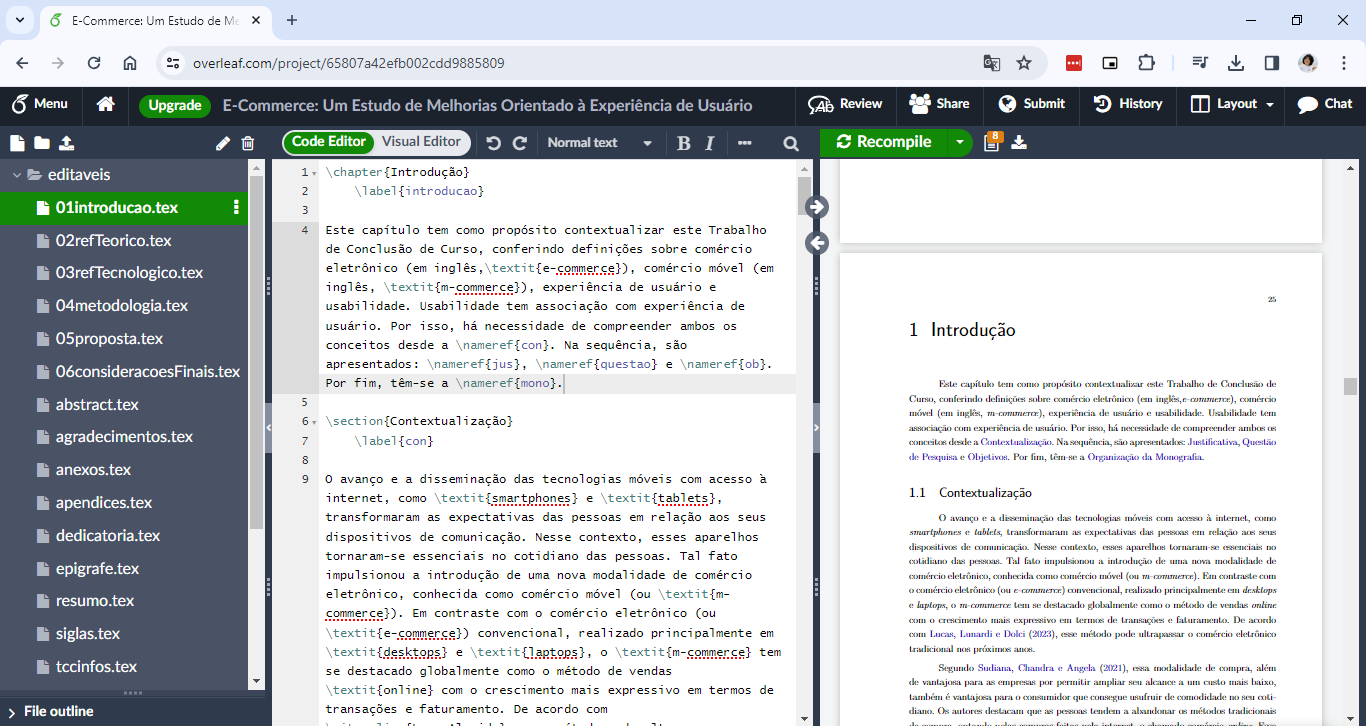
\includegraphics[keepaspectratio=true,scale=0.4]{figuras/cap03overleaf.png}
    \legend{Fonte: Autora}
    \label{fig05}
\end{figure}


%%%%%%%%%%%%%%%%%%%%%%%%%%%%%%%%%%%%%%%%%%%%%%%%%%%%

\section{Apoio Complementar} \label{complementar}

Outros suportes utilizados para concretização do trabalho compreendem: Ferramentas de Comunicação, Ferramentas de Modelagem de Processos e Ferramentas de Versionamento e Hospedagem.

\subsection{Ferramentas de Comunicação}

Para manter a comunicação com a orientadora para revisões, dúvidas e andamento do trabalho, estão sendo utilizadas as ferramentas:
\begin{itemize}
    \item \textbf{Slack}: para manter os rastros dos orientações;
    \item \textbf{Teams}: para reuniões semanais, e
    \item \textbf{Telegram}: para mensagens rápidas entre autora e orientadora.
\end{itemize}

\subsection{Ferramentas de Modelagem de Processos}

O LucidChart é uma plataforma \textit{online} de criação de diagramas e fluxogramas, utilizada para visualizar e comunicar ideias de forma clara e eficiente. Com uma interface intuitiva e uma variedade de modelos e ferramentas de edição, o Lucidchart permite aos usuários criar de diagramas, incluindo organogramas, diagramas de fluxo de processo, mapas mentais, diagramas de rede e muito mais \cite{LucidChart}.

A ferramenta está sendo utilizada para modelagem de processos inerentes à apresentação da metodologia do trabalho. Exemplos desses modelos podem ser encontrados no \hyperref[chap:Metodologia]{Capítulo 4 - Metodologia}.

\subsection{Ferramentas de Versionamento e Hospedagem} 

O Git é um sistema de controle de versão distribuído amplamente utilizado para rastrear as alterações em arquivos de código-fonte durante o desenvolvimento de software. Ele permite que múltiplos desenvolvedores trabalhem em um mesmo projeto simultaneamente, gerenciando suas próprias versões do código e mesclando as alterações de forma eficiente. O Git é conhecido por sua velocidade, eficiência e capacidade de lidar com projetos de todos os tamanhos \cite{Git}.

O GitHub, por outro lado, é uma plataforma de hospedagem de código baseada na web que utiliza o Git para controle de versão. Ele permite que os desenvolvedores armazenem, compartilhem e colaborem em projetos de software de maneira eficiente. Além disso, o GitHub oferece recursos adicionais, como rastreamento de problemas, solicitações de \textit{pull} e integração contínua, tornando-o uma ferramenta valiosa para equipes de desenvolvimento colaborarem em projetos de código aberto ou privados \cite{GitHub}.

\begin{figure}[ht]
    \centering
    \caption{Visão do Repositório no Overleaf}
    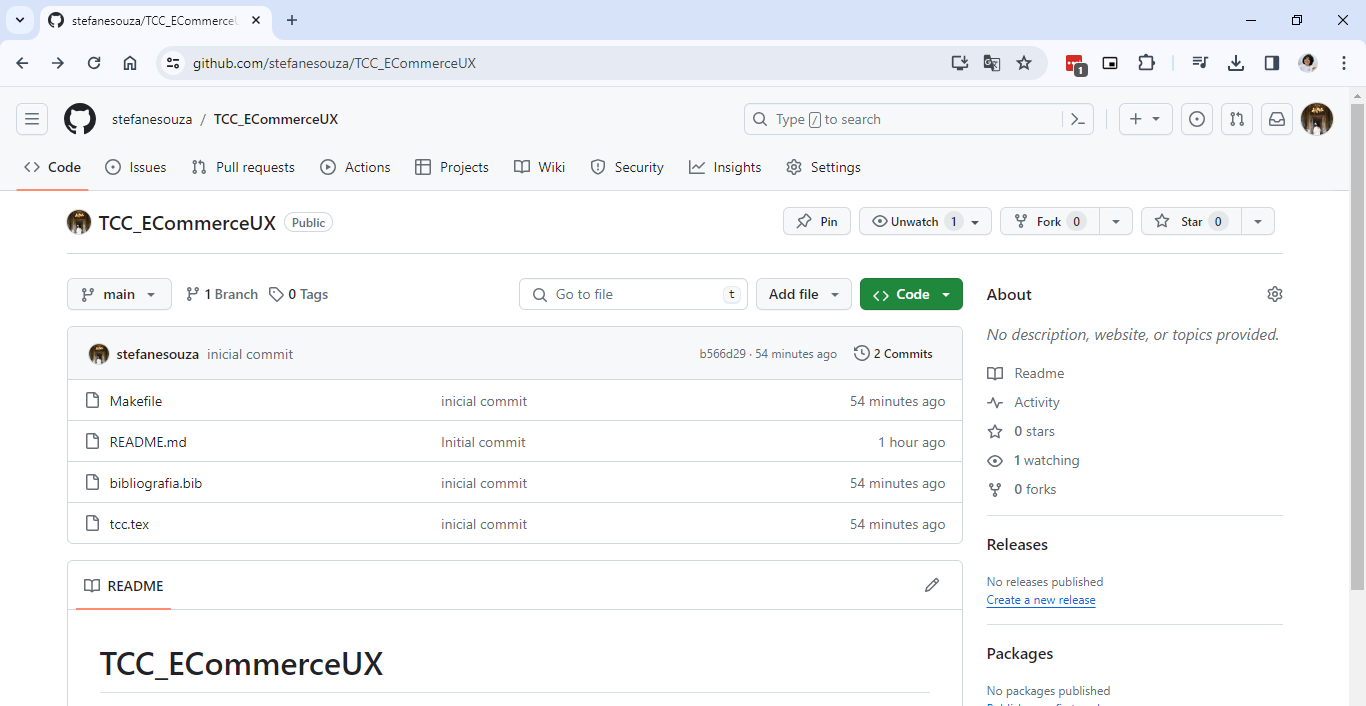
\includegraphics[keepaspectratio=true,scale=0.4]{figuras/cap03github.png}
    \legend{Fonte: Autora}
    \label{fig06}
\end{figure}

%%%%%%%%%%%%%%%%%%%%%%%%%%%%%%%%%%%%%%%%%%%%%%%%%%%%

\section{Resumo do Capítulo} 
    \label{resumo}

Este capítulo abordou as ferramenta de apoio em cada etapa deste Trabalho de Conclusão de Curso, desde a pesquisa e a coleta de dados até ferramenta de prototipação e outros. O Quadro \ref{FerramentasTecnologicas} mostra um resumo das tecnologias utilizadas, assim como seus endereços eletrônicos e versões.

\setfloatlocations{quadro}{hbtp}
\begin{quadro}
\caption{\label{FerramentasTecnologicas}Resumo das Ferramentas Tecnológicas Utilizadas}
\centering

\begin{tabular}{|p{2.5cm}|p{5cm}|p{1.7cm}|p{6.4cm}|}
\hline
\textbf{Nome} & \textbf{Descrição} & \textbf{Versão} & \textbf{Link}                    \\ \hline
Figma                  & Ferramenta de \textit{design} colaborativo & 116.15.15                   & \href{https://www.figma.com}{<https://www.figma.com>} \par Acessado em: 10 fev. 2024 \\ \hline
Git                    & Sistema de controle de versão & 2.44.0                   & \href{https://git-scm.com}{<https://git-scm.com>} \par Acessado em: 05 mar. 2024 \\ \hline
GitHub                 & Plataforma de hospedagem de código & -                   & \href{https://github.com}{<https://github.com>} \par Acessado em: 05 mar. 2024 \\ \hline
Google \textit{Forms}           & Ferramenta de criação de formulários & -                   & \href{https://www.google.com/forms}{<https://www.google.com/forms>} \par Acessado em: 05 mar. 2024 \\ \hline
Google \textit{Sheets}          & Planilhas \textit{online} do Google & -                   & \href{https://www.google.com/sheets}{<https://www.google.com/sheets>} \par Acessado em: 05 mar. 2024 \\ \hline
LucidChart             & Ferramenta de criação de diagramas & -                   & \href{https://www.lucidchart.com}{<https://www.lucidchart.com>} \par Acessado em: 17 fev. 2024 \\ \hline
Microsoft Teams        & Plataforma de colaboração e comunicação & -                   & \href{https://www.microsoft.com/pt-br/microsoft-365/microsoft-teams/group-chat-software}{<https://www.microsoft.com/pt-br/microsoft-365/microsoft-teams/group-chat-software>} \par Acessado em: 09 mar. 2024 \\ \hline
Notion                 & Plataforma de organização e colaboração & 3.2.1                   & \href{https://www.notion.so}{<https://www.notion.so>} \par Acessado em: 10 mar. 2024 \\ \hline
Overleaf               & Editor de LaTeX \textit{online} & abnTeX2                   & \href{https://www.overleaf.com}{<https://www.overleaf.com>} \par Acessado em: 11 mar. 2024 \\ \hline
Slack                  & Plataforma de comunicação em equipe & -                   & \href{https://slack.com}{<https://slack.com>} \par Acessado em: 11 mar. 2024 \\ \hline
Telegram               & Aplicativo de mensagens instantâneas & -                   & \href{https://telegram.org}{<https://telegram.org>} \par Acessado em: 11 mar. 2024 \\ \hline
Trello               & Plataforma de organização de trabalho & -                   & \href{https://https://trello.com/}{<https://https://trello.com/>} \par Acessado em: 11 mar. 2024 \\ \hline
\end{tabular}

\legend{Fonte: Autora}
\end{quadro} 